\documentclass{article}


\usepackage{arxiv}

\usepackage[utf8]{inputenc} % allow utf-8 input
\usepackage[T1]{fontenc}    % use 8-bit T1 fonts
\usepackage{hyperref}       % hyperlinks
\usepackage{url}            % simple URL typesetting
\usepackage{booktabs}       % professional-quality tables
\usepackage{amsfonts}       % blackboard math symbols
\usepackage{nicefrac}       % compact symbols for 1/2, etc.
\usepackage{microtype}      % microtypography
\usepackage{xcolor}      % microtypography
\usepackage{amsmath} % assumes amsmath package installed
\usepackage{amssymb}  % assumes amsmath package installed
\usepackage{epsfig} % for postscript graphics files
\usepackage{mathtools}

\title{Notes}


\author{
  S. Boersma\\ %\thanks{ }
  Supergrid-Institute\\
  Villeurbanne, France \\
  \texttt{sjoerd.boersma@supergrid-institute.com} \\
}

\begin{document}
\maketitle

\begin{abstract}
	This document provides background information on different topics related to the project.
\end{abstract}


% keywords can be removed
%\keywords{}

\section{Problem Formulation}
We are considering the setup as defined in Fig.~\ref{fig:setup}.


\begin{figure}[h]
	\centering
	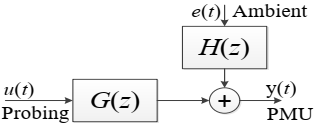
\includegraphics[width=.5\linewidth]{Images/setup}
	\label{fig:setup}
\end{figure}

In this setting we have $G$ defined as the true plant and $H$ as the true noise model. The probing signal $u(t)$ can be chosen by the user and the measurement $y(t)$ can be used for this. The signal $e(t)$ is ambient noise and unknown except that is is assumed to be white Gaussian.   

We want to solve the following optimization problem:
\begin{equation}
\begin{aligned}
\min_{\Phi_u(i\omega)} \qquad & \frac{c_1}{2\pi} \underbrace{\int_{-\pi}^{\pi} \Phi_u(i\omega) \text{d}\omega}_{J_1} + \frac{c_2}{2\pi} \underbrace{\int_{-\pi}^{\pi} |G(i\omega)| \Phi_u(i\omega) \text{d}\omega}_{J_2}, \\
& \text{s.t.} \qquad \text{variance}(\zeta_i) < \varepsilon.
\label{eq:optimalinputdesign1}
\end{aligned}
\end{equation}
The first term in the cost $J_1$ represents the power in the probing signal while he second term in the cost $J_2$ represents the deviation of the measured signal due to probing. The scalars $c_1,c_2,\varepsilon$ are variables that can be chosen by he user. The constraint $\text{variance}(\zeta_i) < \varepsilon$ means that there is an upperbound on the variance of the damping coefficient of mode $i=1,2,\ldots,l$. Solving the problem defined in~\eqref{eq:optimalinputdesign1} results in a $\Phi^*_u(i\omega)$, the optimal spectrum of the probing signal that needs to be transformed to a time domain signal and consequently needs to be applied in the following system identification batch.    

Define the class of input signals as:
\begin{equation}
u(t) = \sum_{r=1}^{M} A_r \cos(\omega_r t + \phi_r), \qquad \Phi_u(i \omega) = \frac{\pi}{2} \sum_{r=1}^{M} A_r^2 \Big( \delta(\omega-\omega_r) + \delta(\omega+\omega_r) \Big). 
\end{equation}

The problem given in~\eqref{eq:optimalinputdesign1} can now be rewritten as:

\begin{equation}
\begin{aligned}
\min_{A_r^2 (r=1,2,,\ldots,,M)} \qquad & \frac{c_1}{2} \sum_{r=1}^{M} A_r^2 + \frac{c_2}{2} \sum_{r=1}^{M} A_r^2 |G_0(i\omega_r,\rho_0)|^2, \\
& \text{s.t.} \qquad \text{variance}(\zeta_i) < \varepsilon,
\label{eq:optimalinputdesign2}
\end{aligned}
\end{equation}
with $G_0(i\omega_r,\rho_0)$ the true system and $\rho_0$ the true parameter vector that contains, among others, the damping coefficients of the critical modes. Obviously both of these are unknown, but the idea is to get estimations via system identification. The information matrix of the parameter vector $\rho$ is defined as:
\begin{equation}
\begin{aligned}
%P_\rho^{-1} = \left( \frac{N}{\sigma_e^2} \frac{1}{2\pi} \int_{-\pi}^{\pi} F_u(i\omega,\rho_0) F^*_u(i\omega,\rho_0) \Phi_u(i\omega) \text{d} \omega \right) + \left( \frac{N}{2\pi} \int_{-\pi}^{\pi} F_e(i\omega,\rho_0) %F^*_e(i\omega,\rho_0) \Phi_u(i\omega) \text{d} \omega \right),
P_\rho^{-1} &= \left( \frac{N}{2\sigma_e^2} \sum_{r=1}^{M} \text{Re} \left\{ F_u(i\omega_r,\rho_0) F^*_u(i\omega_r,\rho_0) \right\} A_r^2 \right) + \left( \frac{N}{2\pi} \int_{-\pi}^{\pi} F_e(i\omega,\rho_0) F^*_e(i\omega,\rho_0) \text{d} \omega \right), \\
            &= \frac{N}{\sigma_e^2} \sum_{r=1}^{M} R_r A_r^2 + N X
\end{aligned}
\label{eq:informationmatrix}
\end{equation}  
where:
\begin{itemize}
	\item $N$ is the number of data points used in the optimization,
	\item $\sigma_e^2$ is the variance of the ambient noise,
	\item $P_\rho$ the covariance matrix of the parameter vector,
	\item $X$ is the solution of the Lyapunov equation $X=CXC^T+DD^T$ with $A,D$ state-space matrices of a realization of $F_e(i\omega)$.  
	\item and the functions $F_u(i\omega,\rho_0)$ and $F_e(i\omega,\rho_0)$ are defined as:
	\begin{equation}
	\begin{aligned}
	 F_u(i\omega_r,\rho_0) &= H^{-1}(i \omega_r,\rho) \frac{\partial G(i\omega_r , \rho )}{\partial \rho} \Bigg|_{\rho=\rho_0} \\
	 F_e(i\omega,\rho_0) &= H^{-1}(i \omega,\rho) \frac{\partial H(i\omega , \rho )}{\partial \rho} \Bigg|_{\rho=\rho_0}.
	\end{aligned}
	\end{equation}
\end{itemize}

Note that 
\begin{equation}
P_\rho(i,i) = \text{var} (\zeta_i), \qquad \text{for} \quad i=1,2,\ldots,n,
\end{equation}
with $n$ the number of critical nodes. We use the above to get the following LMI:
\begin{equation}
\begin{pmatrix} \varepsilon & e_i^T \\ e_i & P_\rho^{-1} \end{pmatrix} > 0,
\end{equation}
with $e_i$ a unit vector with one on its $i^{\text{th}}$ element (corresponding to the $i^{\text{th}}$ damping coefficient). This LMI defines a bound $\varepsilon$ on the variance of the damping coefficient.

This leads to the final optimization problem:
\begin{equation}
\begin{aligned}
\min_{A_r^2 (r=1,2,,\ldots,,M)} \qquad & \frac{c_1}{2} \sum_{r=1}^{M} A_r^2 + \frac{c_2}{2} \sum_{r=1}^{M} A_r^2 |G_0(i\omega_r,\rho_0)|^2, \\
& \text{s.t.} \qquad \begin{pmatrix} \varepsilon & e_i^T \\ e_i & P_\rho^{-1} \end{pmatrix} > 0, \quad \text{and} \quad A_r^2 \geq 0, \quad \text{for} \quad r=1,2,\ldots,M.
\label{eq:optimalinputdesign3}
\end{aligned}
\end{equation}
Indeed the true parameter vector $\rho_0$ will be estimated using system identification techniques. We need the following expression: $P_\rho$, hence we need $\hat{G}(i\omega,\hat{\rho}), \hat{H}(i\omega,\hat{\rho}), \frac{\partial \hat{G}(i\omega,\rho)}{\partial \rho}, \frac{\partial \hat{H}(i\omega,\rho)}{\partial \rho}$. Note that the parameter vector should contain the critical damping coefficients, which is not standard. In other words, we need to find a parameterization of $G(i\omega),H(i\omega)$ in terms of, among others, the critical damping coefficients.  

\section{Parameterization ARMAX in terms of the damping coefficients}

The parameterization presented in~\eqref{eq:ARMAX_t} is in terms of the parameter vector $\theta$. However, we would like to have a parameterization in terms of, among others, the damping coefficients of the ARMAX model. These damping coefficients are defined as $\zeta_i$ for $i=1,2,\ldots,n_a$ and hence should be contained in the complete parameter vector $\rho$. In other words, we want a following transfer function representation
\begin{equation}
\begin{aligned}
Y(z) = &\underbrace{\frac{  \theta_{n_a+1} z^{n_b-1} + \theta_{n_a+2} z^{n_b-2} + \dots + \theta_{n_a+n_b}}{(z^{n_a} + \theta_1 z^{n_a-1} + \dots + \theta_{n_a} )z^{-n_k} }}_{G(z,\theta)} U(z) + \ldots \\
&\ldots \underbrace{\frac{ z^{n_c} + \theta_{n_a+n_b+1}  z^{n_c-1} + \dots + \theta_{n_a+n_b+n_c} }{z^{n_a} + \theta_1 z^{n_a-1} + \dots + \theta_{n_a}}}_{H(z,\theta)} E(z),
\label{eq:ARMAX_z_theta}
\end{aligned}
\end{equation}
with $z \in \mathbb{C}$, parameter vector $\theta = \begin{pmatrix} \theta_1 & \theta_2 & \dots & \theta_{n_a} & \theta_{n_a+1} & \theta_{n_a+n_b+n_c} \end{pmatrix}^T \in \mathbb{R}^{n_a+n_b+n_c}$, $Y(z),U(z),E(z)$ the $z$-transform of the output, input and noise, respectively. The positive scalars $n_a,n_b,n_c$ are variables that need to be defined by the user and depend on the application under consideration. The above equation can be written as:
\begin{equation}
\begin{aligned}
Y(z) = &\underbrace{\frac{  (\theta_{n_a+1} z^{n_b-1} + \theta_{n_a+2} z^{n_b-2} + \dots + \theta_{n_a+n_b})z^{-n_k}}{   \prod_{i=1, i \neq j}^{n_i} \left( z^2 - 2 e^{-\zeta_i w_{n,i} h } \cos (w_{n,i} \sqrt{1-\zeta_i^2} h) z + e^{-2 \zeta_i w_{n,i} h}  \right)  \prod_{j=1, j \neq i}^{n_r} \left(  z-\text{sign}(z_r)e^{-\omega_{n,j}h} \right) }}_{G(z,\theta)} U(z) + \ldots \\
&\ldots \underbrace{\frac{ z^{n_c} + \theta_{n_a+n_b+1}  z^{n_c-1} + \dots + \theta_{n_a+n_b+n_c} }{       \prod_{i=1, i \neq j}^{n_i} \left( z^2 - 2 e^{-\zeta_i w_{n,i} h } \cos (w_{n,i} \sqrt{1-\zeta_i^2} h) z + e^{-2 \zeta_i w_{n,i} h}  \right)  \prod_{j=1, j \neq i}^{n_r} \left(  z-\text{sign}(z_r)e^{-\omega_{n,j}h} \right)      }}_{H(z,\theta)} E(z),
\label{eq:ARMAX_z_zeta}
\end{aligned}
\end{equation}
with $z_r$ the real valued pole. We assume $H(z)$ to be monic. Define a new parameter vector:
\begin{equation}
\begin{aligned}
\theta  &= \begin{pmatrix} \omega_{n,1} & \ldots & \omega_{n,n_r} & \omega_{n,n_r+1} & \zeta_{n_r+1} & \ldots & \omega_{n,n_r+n_i} & \zeta_{n_r+n_i} & \theta_{2n_i+n_r+1} \ldots & \theta_{2n_i+n_r+n_b+n_c} \end{pmatrix}^T \in \mathbb{R}^{2n_i+n_r+n_b+n_c}, \\
\theta &= \begin{pmatrix} \rho^T & \tilde{\theta}^T \end{pmatrix}^T, \nonumber
\end{aligned}
\end{equation}
with $n_i$ the number of complex pole pairs and $n_r$ the number of real valued poles and the relation $2n_i+n_r=n_a$. Define a two row vector containing a monomial basis:
\begin{equation}
\begin{aligned}
m(z) &= \begin{pmatrix} z^{n_a} & z^{n_a-1} & \dots & z & 1 \end{pmatrix} \in \mathbb{R}^{1 \times n_a+1}
\end{aligned}
\end{equation} 
and characteristic polynomial as:
\begin{equation}
\begin{aligned}
p(z,\rho) &= \prod_{i=1, i \neq j}^{n_i} \left( z^2 - 2 e^{-\zeta_i w_{n,i} h } \cos (w_{n,i} \sqrt{1-\zeta_i^2} h) z + e^{-2 \zeta_i w_{n,i} h}  \right)  \prod_{j=1, j \neq i}^{n_r} \left(  z- \text{sign}(z_r) e^{-\omega_{n,j}h} \right),
\end{aligned}
\end{equation}
so that we can write:
\begin{equation}
\begin{aligned}
G(z,\theta) = m(z) \underbrace{\begin{pmatrix} 0_{n_a-n_b} \\ \theta_{n_a+1}  \\ \vdots \\ \theta_{n_a+n_b} \end{pmatrix}}_{B_1(\tilde{\theta})} p(z,\rho)^{-1} z^{-n_k}, \qquad H(z,\theta) =   m(z) \underbrace{\begin{pmatrix}  1 \\  \theta_{n_a+n_b+1}  \\ \vdots \\ \theta_{n_a+n_b+n_c} \end{pmatrix}}_{B_2(\tilde{\theta})} p(z,\rho)^{-1}.
\end{aligned}
\end{equation}

The derivative of $G(z)$ with respect to the parameter vector is then defined as follows:
\begin{equation}
\begin{aligned}
\frac{\partial G(z,\theta)}{\partial \theta} &= 
\left(\begin{array}{c} 
\dfrac{\partial G(z,\theta)}{\partial \omega_{n,1}} \\
\vdots \\
\dfrac{\partial G(z,\theta)}{\partial \omega_{n,n_r}} \\
\dfrac{\partial G(z,\theta)}{\partial \omega_{n,n_r+1}} \\ \dfrac{\partial G(z,\theta)}{\partial \zeta_{n_r+1}} \\ \vdots \\ \dfrac{\partial G(z,\theta)}{\partial \omega_{n,n_r+n_i}} \\ \dfrac{\partial G(z,\theta)}{\partial \zeta_{n_r+n_i}} \\ \hline \dfrac{\partial G(z,\theta)}{\partial \theta_{n_a + 1}} \\ \dfrac{\partial G(z,\theta)}{\partial \theta_{n_a + 2}} \\ \vdots \\ \dfrac{\partial G(z,\theta)}{\partial \theta_{n_a + n_b }} \\ \hline \dfrac{\partial G(z,\theta)}{\partial \theta_{n_a + n_b + 1}} \\ \vdots \\ \dfrac{\partial G(z,\theta)}{\partial \theta_{n_a + n_b + n_c}} 
\end{array} \right)
= 
\left(\begin{array}{c} 
\dfrac{\partial p(z,\rho)^{-1}}{\partial \omega_{n,1}} m(z) B_1(\tilde{\theta}) \\ 
\vdots \\
\dfrac{\partial p(z,\rho)^{-1}}{\partial \omega_{n,n_r}} m(z) B_1(\tilde{\theta}) \\ 
\dfrac{\partial p(z,\rho)^{-1}}{\partial \omega_{n,n_r+1}} m(z) B_1(\tilde{\theta}) \\  
\dfrac{\partial p(z,\rho)^{-1}}{\partial \zeta_{n_r+1}} m(z) B_1(\tilde{\theta}) \\ 
\vdots \\ 
\dfrac{\partial p(z,\rho)^{-1}}{\partial \omega_{n,n_r+n_i}} m(z) B_1(\tilde{\theta}) \\  
\dfrac{\partial p(z,\rho)^{-1}}{\partial \zeta_{n_r+n_i}} m(z) B_1(\tilde{\theta}) \\  
\hline p(z,\rho)^{-1} m(z) \dfrac{\partial B_1(\tilde{\theta})}{\partial \theta_{n_a+1}} \\ 
p(z,\rho)^{-1} m(z) \dfrac{\partial B_1(\tilde{\theta})}{\partial \theta_{n_a+2}} \\ 
\vdots \\  
p(z,\rho)^{-1} m(z) \dfrac{\partial B_1(\tilde{\theta})}{\partial \theta_{n_a+n_b}} \\ 
\hline 0 \\ 
\vdots \\ 
0
\end{array} \right) z^{-n_k} 
= 
\left(\begin{array}{c} 
-p(z,\rho)^{-2} \dfrac{\partial p(z,\rho)}{\partial \omega_{n,1}} m(z) B_1(\tilde{\theta}) \\  
\vdots \\
-p(z,\rho)^{-2} \dfrac{\partial p(z,\rho)}{\partial \omega_{n,n_r}} m(z) B_1(\tilde{\theta}) \\  
-p(z,\rho)^{-2} \dfrac{\partial p(z,\rho)}{\partial \omega_{n,n_r+1}} m(z) B_1(\tilde{\theta}) \\  
-p(z,\rho)^{-2}\dfrac{\partial p(z,\rho)}{\partial \zeta_{n_r+1}} m(z) B_1(\tilde{\theta}) \\ 
\vdots \\ 
-p(z,\rho)^{-2}\dfrac{\partial p(z,\rho)}{\partial \omega_{n,n_r+1+n_i}} m(z) B_1(\tilde{\theta}) \\  
-p(z,\rho)^{-2}\dfrac{\partial p(z,\rho)}{\partial \zeta_{n_r+1+n_i}} m(z) B_1(\tilde{\theta}) \\  
\hline p(z,\rho)^{-1} m(z) \dfrac{\partial B_1(\tilde{\theta})}{\partial \theta_{n_a+1}} \\ 
p(z,\rho)^{-1} m(z) \dfrac{\partial B_1(\tilde{\theta})}{\partial \theta_{n_a+2}} \\ 
\vdots \\  
p(z,\rho)^{-1} m(z) \dfrac{\partial B_1(\tilde{\theta})}{\partial \theta_{n_a+n_b}} \\ 
\hline 0 \\ 
\vdots \\ 
0
\end{array} \right) z^{-n_k} \nonumber
\end{aligned}
\end{equation}

\clearpage
The derivative of $H(z)$ with respect to the parameter vector is then defined as follows:
\begin{equation}
\begin{aligned}
\frac{\partial H(z,\theta)}{\partial \theta} &= 
\left(\begin{array}{c} 
\dfrac{\partial H(z,\theta)}{\partial \omega_{n,1}} \\
\vdots \\
\dfrac{\partial H(z,\theta)}{\partial \omega_{n,n_r}} \\
\dfrac{\partial H(z,\theta)}{\partial \omega_{n,n_r+1}} \\ \dfrac{\partial H(z,\theta)}{\partial \zeta_{n_r+1}} \\ \vdots \\ \dfrac{\partial H(z,\theta)}{\partial \omega_{n,n_r+n_i}} \\ \dfrac{\partial H(z,\theta)}{\partial \zeta_{n_r+n_i}} \\ \hline \dfrac{\partial H(z,\theta)}{\partial \theta_{n_a + 1}} \\ \dfrac{\partial H(z,\theta)}{\partial \theta_{n_a + 2}} \\ \vdots \\ \dfrac{\partial H(z,\theta)}{\partial \theta_{n_a + n_b }} \\ \hline \dfrac{\partial H(z,\theta)}{\partial \theta_{n_a + n_b + 1}} \\ \vdots \\ \dfrac{\partial H(z,\theta)}{\partial \theta_{n_a + n_b + n_c}} 
\end{array} \right)
= 
\left(\begin{array}{c} 
\dfrac{\partial p(z,\rho)^{-1}}{\partial \omega_{n,1}} m(z) B_2(\tilde{\theta}) \\ 
\vdots \\
\dfrac{\partial p(z,\rho)^{-1}}{\partial \omega_{n,n_r}} m(z) B_2(\tilde{\theta}) \\ 
\dfrac{\partial p(z,\rho)^{-1}}{\partial \omega_{n,n_r+1}} m(z) B_2(\tilde{\theta}) \\  
\dfrac{\partial p(z,\rho)^{-1}}{\partial \zeta_{n_r+1}} m(z) B_2(\tilde{\theta}) \\ 
\vdots \\ 
\dfrac{\partial p(z,\rho)^{-1}}{\partial \omega_{n,n_r+n_i}} m(z) B_2(\tilde{\theta}) \\  
\dfrac{\partial p(z,\rho)^{-1}}{\partial \zeta_{n_r+n_i}} m(z) B_2(\tilde{\theta}) \\  
\hline 0 \\ 
\vdots \\ 
0 \\
\hline p(z,\rho)^{-1} m(z) \dfrac{\partial B_2(\tilde{\theta})}{\partial \theta_{n_a+n_b+1}} \\ 
p(z,\rho)^{-1} m(z) \dfrac{\partial B_2(\tilde{\theta})}{\partial \theta_{n_a+n_b+2}} \\ 
\vdots \\  
p(z,\rho)^{-1} m(z) \dfrac{\partial B_2(\tilde{\theta})}{\partial \theta_{n_a+n_b+n_c}} \\ 
\end{array} \right)
= 
\left(\begin{array}{c} 
-p(z,\rho)^{-2} \dfrac{\partial p(z,\rho)}{\partial \omega_{n,1}} m(z) B_2(\tilde{\theta}) \\  
\vdots \\
-p(z,\rho)^{-2} \dfrac{\partial p(z,\rho)}{\partial \omega_{n,n_r}} m(z) B_2(\tilde{\theta}) \\  
-p(z,\rho)^{-2} \dfrac{\partial p(z,\rho)}{\partial \omega_{n,n_r+1}} m(z) B_2(\tilde{\theta}) \\  
-p(z,\rho)^{-2}\dfrac{\partial p(z,\rho)}{\partial \zeta_{n_r+1}} m(z) B_2(\tilde{\theta}) \\ 
\vdots \\ 
-p(z,\rho)^{-2}\dfrac{\partial p(z,\rho)}{\partial \omega_{n,n_r+1+n_i}} m(z) B_2(\tilde{\theta}) \\  
-p(z,\rho)^{-2}\dfrac{\partial p(z,\rho)}{\partial \zeta_{n_r+1+n_i}} m(z) B_2(\tilde{\theta}) \\  
\hline 0 \\ 
\vdots \\ 
0 \\
\hline p(z,\rho)^{-1} m(z) \dfrac{\partial B_2(\tilde{\theta})}{\partial \theta_{n_a+n_b+1}} \\ 
p(z,\rho)^{-1} m(z) \dfrac{\partial B_2(\tilde{\theta})}{\partial \theta_{n_a+n_b+2}} \\ 
\vdots \\  
p(z,\rho)^{-1} m(z) \dfrac{\partial B_2(\tilde{\theta})}{\partial \theta_{n_a+n_b+n_c}} \\ 
\end{array} \right) \nonumber
\end{aligned}
\end{equation}
with
\begin{equation}
\dfrac{\partial p(z,\rho)}{\partial \omega_{n,i}} = \begin{dcases*} \text{sign}(z_r) h e^{-\omega_{n,i}h}, & for $\quad i=1,\ldots,n_r$, \\
f_1(\rho), & for $\quad i=n_i+1,\ldots,n_i+n_r$, 
\end{dcases*} 				 	
\end{equation}
and
\begin{equation}
\dfrac{\partial p(z,\rho)}{\partial \zeta_{i}} =  	f_2(\rho), \quad \text{for} \quad i=n_i+1,\ldots,n_i+n_r,    
\end{equation}


%%%%%%%%%%%%%%%%%%%%%%%%%%%%%%%%%%%%%%%%%%%%%%%%%%%%%%%%%%%%%%%%%%%%%%%%%%%%%%%%%%%%%%%%%%%%%%%%%
%%%%%%%%%%%%%%%%%%%%%%%%%%%%%%%%%%%%%%%%%%%%%%%%%%%%%%%%%%%%%%%%%%%%%%%%%%%%%%%%%%%%%%%%%%%%%%%%%
%%%%%%%%%%%%%%%%%%%%%%%%%%%%%%%%%%%%%%%%%%%%%%%%%%%%%%%%%%%%%%%%%%%%%%%%%%%%%%%%%%%%%%%%%%%%%%%%%


%\clearpage
%\section{Parameterization ARMAX in parameter vector $\theta$ (does not work when $na=nc$)}
%Define the following ARMAX model as transfer function:
%
%\begin{equation}
%\begin{aligned}
%Y(z) = &\underbrace{\frac{  \theta_{n_a+1} z^{n_b-1} + \theta_{n_a+2} z^{n_b-2} + \dots + \theta_{n_a+n_b}}{z^{n_a} + \theta_1 z^{n_a-1} + \dots + \theta_{n_a}}}_{G(z,\theta)} U(z) + \ldots \\
%		 &\ldots \underbrace{\frac{ z^{n_c} + \theta_{n_a+n_b+1}  z^{n_c-1} + \dots + \theta_{n_a+n_b+n_c} }{z^{n_a} + \theta_1 z^{n_a-1} + \dots + \theta_{n_a}}}_{H(z,\theta)} E(z),
%		 \label{eq:ARMAX_z}
%\end{aligned}
%\end{equation}
%with $z \in \mathbb{C}$, parameter vector $\theta = \begin{pmatrix} \theta_1 & \theta_2 & \dots & \theta_{n_a+n_b+n_c} \end{pmatrix}^T \in \mathbb{R}^{n_a+n_b+n_c}$, $Y(z),U(z),E(z)$ the $z$-transform of the output, input and noise, respectively. The positive scalars $n_a,n_b,n_c$ are variables that need to be defined by the user and depend on the application under consideration.
%
%A state-space realization of~\eqref{eq:ARMAX_z} is defined as follows:
%
%\begin{equation}
%\begin{aligned}
%x_{k+1} &= 
%\underbrace{\begin{pmatrix} -\theta_1 & -\theta_2 & -\theta_3 & \dots & -\theta_{n_a} \\ 
%                    1 & 0 & 0 & \dots & 0 \\
%                    0 & 1 & 0 & \dots & 0  \\
%                     &   & \ddots &  &  \\
%                    0 &  0 & \dots & 1 & 0 \end{pmatrix}^T}_{A(\theta)} x_k + \underbrace{\begin{pmatrix} 0_{n_a-n_b} & 0_{n_a-n_c-1} \\ \theta_{n_a+1} & 1 \\ \theta_{n_a+2} & \theta_{n_a+n_b+1}  \\ \vdots & \vdots \\ \theta_{n_a+n_b} & \theta_{n_a+n_b+n_c} \end{pmatrix}}_{B(\theta)} \begin{pmatrix} u_k \\ e_k \end{pmatrix} \\
%y_k     &= \underbrace{\begin{pmatrix} 1 & 0 & \dots & 0 \end{pmatrix}}_{C} x_k + \underbrace{\begin{pmatrix} D_u & I \end{pmatrix}}_{D} \begin{pmatrix} u_k \\ e_k \end{pmatrix},
%		 \label{eq:ARMAX_t}
%\end{aligned}
%\end{equation}  
%with $0_{n}$ a zero valued column vector of length $n$, i.e., $0_n \in \mathbb{R}^{n \times 1}$. We have the following relations:
%\begin{equation}
%G(z,\theta) = C \Big( z I_{n_a} - A(\theta) \Big)^{-1} B_1(\theta) + D_u, \qquad H(z,\theta) = C \Big( z I_{n_a} - A(\theta) \Big)^{-1} B_2(\theta) + I,
%\end{equation}
%with $B_i(\theta)$ the $i^{\text{th}}$ column of the matrix $B(\theta)$ as defined in~\eqref{eq:ARMAX_t}. Also define a row vector containing a monomial basis:
%\begin{equation}
%m(z) = \begin{pmatrix} z^{n_a-1} & z^{n_a-2} & \dots & z & 1 \end{pmatrix} \in \mathbb{R}^{1 \times n_a}
%\end{equation} 
%and characteristic polynomial as:
%\begin{equation}
%p(z) = z^{n_a} + \theta_1 z^{n_a-1} + \dots + \theta_{n_a}
%\end{equation}
%
%The derivative of $G(z,\theta)$ with respect to the parameter vector $\theta$ is defined as:
%\begin{equation}
%\begin{aligned}
%\frac{\partial G(z,\theta)}{\partial \theta} &= 
%\left(\begin{array}{c} 
%\frac{\partial G(z,\theta)}{\partial \theta_1} \\ \frac{\partial G(z,\theta)}{\partial \theta_2} \\ \vdots \\ \frac{\partial G(z,\theta)}{\partial \theta_{n_a}} \\ \hline \frac{\partial G(z,\theta)}{\partial \theta_{n_a + 1}} \\ \frac{\partial G(z,\theta)}{\partial \theta_{n_a + 2}} \\ \vdots \\ \frac{\partial G(z,\theta)}{\partial \theta_{n_a + n_b }} \\ \hline \frac{\partial G(z,\theta)}{\partial \theta_{n_a + n_b + 1}} \\ \vdots \\ \frac{\partial G(z,\theta)}{\partial \theta_{n_a + n_b + n_c}} 
%\end{array} \right)
%= 
%\left(\begin{array}{c} 
%- z^{n_a-1} p(z)^{-2} m(z) B_1(\theta) \\  - z^{n_a-2} p(z)^{-2} m(z) B_1(\theta) \\ \vdots \\ - p(z)^{-2} m(z) B_1(\theta) \\ \hline p(z)^{-1} m(z) \dfrac{\partial B_1(\theta)}{\partial \theta_{n_a+1}} \\ p(z)^{-1} m(z) \dfrac{\partial B_1(\theta)}{\partial \theta_{n_a+2}} \\ \vdots \\  p(z)^{-1} m(z) \dfrac{\partial B_1(\theta)}{\partial \theta_{n_a+n_b}} \\ \hline 0 \\ \vdots \\ 0
%\end{array} \right). 
%\end{aligned}
%\end{equation}
%
%The derivative of $H(z,\theta)$ with respect to the parameter vector $\theta$ is defined as:
%\begin{equation}
%\begin{aligned}
%\frac{\partial H(z,\theta)}{\partial \theta} &= 
%\left(\begin{array}{c} 
%\frac{\partial H(z,\theta)}{\partial \theta_1} \\ \frac{\partial H(z,\theta)}{\partial \theta_2} \\ \vdots \\ \frac{\partial H(z,\theta)}{\partial \theta_{n_a}} \\ \hline \frac{\partial H(z,\theta)}{\partial \theta_{n_a + 1}} \\  \vdots \\ \frac{\partial H(z,\theta)}{\partial \theta_{n_a + n_b }} \\ \hline \frac{\partial H(z,\theta)}{\partial \theta_{n_a + n_b + 1}} \\ \frac{\partial H(z,\theta)}{\partial \theta_{n_a + n_b + 2}} \\ \vdots \\ \frac{\partial H(z,\theta)}{\partial \theta_{n_a + n_b + n_c}} 
%\end{array} \right)
%= 
%\left(\begin{array}{c} 
%- z^{n_a-1} p(z)^{-2} m(z) B_2(\theta) \\  - z^{n_a-2} p(z)^{-2} m(z) B_2(\theta) \\ \vdots \\ - p(z)^{-2} m(z) B_2(\theta) \\ \hline 0 \\ \vdots \\ 0 \\ \hline p(z)^{-1} m(z) \dfrac{\partial B_2(\theta)}{\partial \theta_{n_a+n_b+1}} \\ p(z)^{-1} m(z) \dfrac{\partial B_2(\theta)}{\partial \theta_{n_a+n_b+2}} \\ \vdots \\  p(z)^{-1} m(z) \dfrac{\partial B_2(\theta)}{\partial \theta_{n_a+n_b+n_c}}
%\end{array} \right) 
%\end{aligned}
%\end{equation}

%
%In state-space representation we then have:
%\begin{equation}
%\begin{aligned}
%x_{k+1} &= A(\rho,\tilde{\theta}) x_k + B(\rho,\tilde{\theta}) \begin{pmatrix} u_k \\ e_k \end{pmatrix} \\
%y_k     &= C x_k.
%\end{aligned}
%\end{equation}  
%Or $C(\rho,\tilde{\theta})$ in combination with constant $B$ is also possible. Define the complete parameter vector now as
%\begin{equation}
%\begin{aligned}
%\theta &= \begin{pmatrix} \zeta_1 & \dots & \zeta_{n_a} & \omega_{n,1} & \dots & \omega_{n,n_a} & \theta_{n_a+1} & \theta_{n_a+2} & \dots & \theta_{n_a+n_b+n_c} \end{pmatrix} \\
%       &= \begin{pmatrix} \rho & \tilde{\theta}   \end{pmatrix},
%\end{aligned}
%\end{equation}
%with natural frequencies $\omega_{n,i}$.

%A state-space realization of~\eqref{eq:ARMAX_z} is defined as follows:
%
%\begin{equation}
%\begin{aligned}
%x_{k+1} &= 
%\underbrace{\begin{pmatrix} -a_1 & -a_2 & -a_3 & \dots & -a_{n_a} \\ 
%	1 & 0 & 0 & \dots & 0 \\
%	0 & 1 & 0 & \dots & 0  \\
%	&   & \ddots &  &  \\
%	0 &  0 & \dots & 1 & 0 \end{pmatrix}^T}_{A(\theta)} x_k + \underbrace{\begin{pmatrix} 0_{n_a-n_b} & 0_{n_a-n_c-1} \\ \theta_{n_a+1} & 1 \\ \theta_{n_a+1} & \theta_{n_a+n_b+1}  \\ \vdots & \vdots \\ \theta_{n_a+n_b} & \theta_{n_a+n_b+n_c} \end{pmatrix}}_{B(\theta)} \begin{pmatrix} u_k \\ e_k \end{pmatrix} \\
%y_k     &= \underbrace{\begin{pmatrix} 1 & 0 & \dots & 0 \end{pmatrix}}_{C} x_k.
%\label{eq:ARMAX_t_zeta}
%\end{aligned}
%\end{equation}  
%Now we note that the coefficients $a_i(\zeta_i,\omega_{n,i})$ depend on the damping coefficient and the natural frequency as follows for a second order system
%\begin{equation}
%a_1 = 2 e^{-\zeta_i w_{n,i} h } \cos (w_{n,i} \sqrt{1-\zeta_i^2} h), \qquad a_2 = e^{-2 \zeta_i w_{n,i} h}
%\end{equation}
%and for a first order system
%
% 
%\section{Parameterization second and first order systems}
%A first and second order system can be defined as follows:
%\begin{equation}
%Y_1(s) = \underbrace{\frac{1}{\frac{1}{\omega_n}s+1}}_{G_1(s)} U_1(s), \qquad Y_2(s) = \underbrace{\frac{w_n^2}{s^2+2 \zeta \omega_n s + \omega_n^2}}_{G_2(s)} U_2(s),
%\end{equation}
%with $\omega_n$ the natural frequency of the transfer and $\zeta$ its damping coefficient. For first order systems, the damping coefficient is equal to one. 





\clearpage
\appendix
\section{Appendix}

\clearpage
\bibliographystyle{unsrt}
%\bibliography{bibliography}

\end{document}
